\documentclass[a4paper]{article}%тип документа


\usepackage{amsmath,amsfonts,amssymb,amsthm,mathtools}
\usepackage{gensymb} 
\usepackage{amssymb}
\usepackage{wasysym}
\usepackage{ mathrsfs }

\usepackage{geometry} % Меняем поля страницы
\geometry{left=2cm}% левое поле
\geometry{right=2cm}% правое поле
\geometry{top=2cm}% верхнее поле
\geometry{bottom=2cm}% нижнее поле

\usepackage[table,xcdraw]{xcolor}%цветовые таблицы
\usepackage{multirow}%несколько столбцов и строк в таблицах
\usepackage{textcomp}%доп. символы


%Русский язык
\usepackage[T2A]{fontenc} %кодировка
\usepackage[utf8]{inputenc} %кодировка исходного кода
\usepackage[english,russian]{babel} %локализация и переносы

%отступы 


%Вставка картинок
\usepackage{graphicx}
\usepackage{wrapfig, caption}
\graphicspath{}
\DeclareGraphicsExtensions{.pdf,.png,.jpg, .jpeg}
\newcommand\ECaption[1]{%
     \captionsetup{font=footnotesize}%
     \caption{#1}}

%Графики
\usepackage{pgfplots}
\pgfplotsset{compat=1.9}

%Математика
\usepackage{amsmath, amsfonts, amssymb, amsthm, mathtools}

%Заголовок
\author{Подлесный Артём \\ группа 827}
\title{Работа 3.4.5 \\ Петля гистерезиса.}




\begin{document}
\maketitle
\section*{Цель работы:} изучение петель гистерезиса ферромагнитных материалов с помощью осциллографа

\section*{В работе используются:} автотрансформатор, понижающий трансформатор, интегрирующая цепочка, амперметр, вольтметр, электронный осциллограф, делитель напряжения, тороидальные образцы с двумя обмотками.

\section*{Общая теория}

\begin{wrapfigure}{l}{0.3\textwidth}
	\vspace{-20pt}
	\begin{center}
		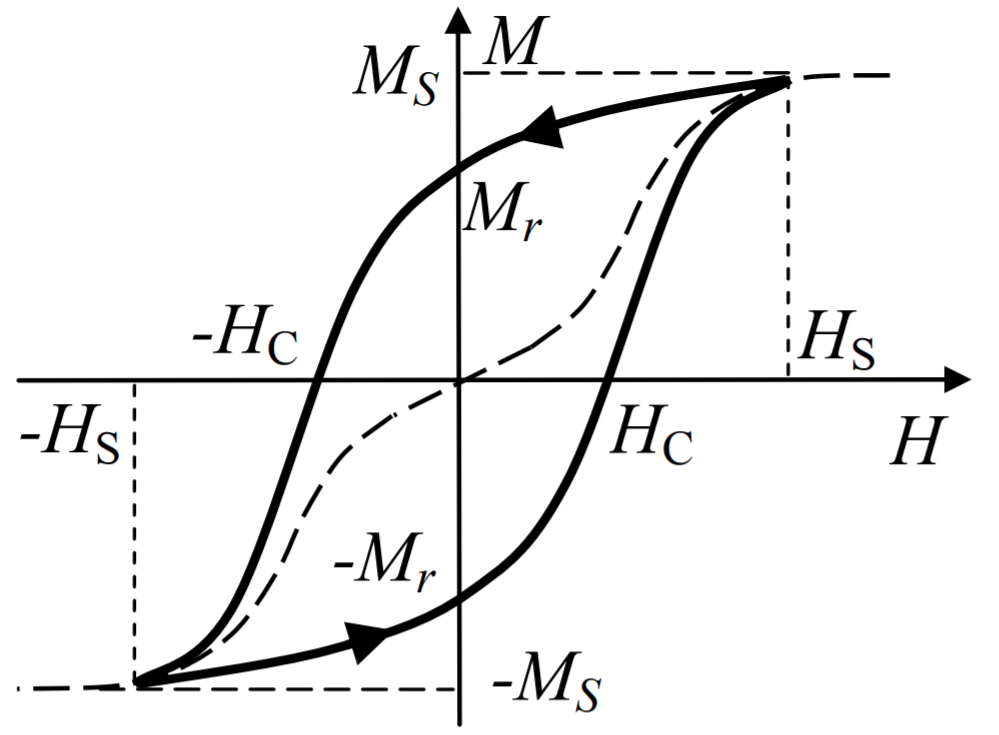
\includegraphics[width=0.3\textwidth]{petl}
	\end{center}
	\vspace{-20pt}
	\caption{Петля гистерезиса}
	\vspace{-10pt}
\end{wrapfigure} 
Рассмотрим большой фрагмет ферромагнетика. Из-за хаотического расположения доменов, его суммарная намагниченность равна нулю. При включении внешеного магнитного поля \textbf{$H$} будет расти объем областей с магнитным моментом \textbf{$I$}, сонаправленным с вектором внешного поля. Этот рост происходит путем смещения границ доменов. Из-за дефектов кристаллической структуры могут происходить необратимые изменения доменных границ. При дальнейшем возрастании  \textbf{$H$}  момент начинает поворачиваться к полю до совпадения, т.е. при некотором значении внешнего поля ферромагнетик ведет себя как один домен с моментом \textbf{$I_{s}$}, направленным по \textbf{$H$}. Это состояние называется состоянием технического насыщения. Петля гистерезиса -- график, описывающий процесс перемагничивания ферромагнетика. Охватывающая точки, соответствующие техническому насыщению, петля называется предельной. 

На графике отмечена коэрцитивная сила \textbf{$H_{c}$}, то есть поле, при котором намагниченность зануляется. Намагниченность \textbf{$M_{r}$}, которая остается, если, предварительно намагнитив ферромагнетик до насыщения, выключить поле, называется остаточной.

Для аналогичного графика зависимости $B(H)$ можно определить соответствующие величины и ввести характеризующую его величину
\begin{equation}
\mu_{max} = \frac{1}{\mu_0}\cdot\frac{dB}{dH}
\end{equation}

\section*{Измерение магнитной индукции и напряженности магнитного поля в образце}

Магнитную индукцию удобно определять с помощью ЭДС, возникающей при изменении потока $\Phi$ в катушке, намотанной на образец:



\begin{equation}
\mathscr{E} = -\frac{d\Phi}{dt} ;
\end{equation}

\begin{equation}
\Phi = BSN;
\end{equation}
Здесь $N$ - число витков в измерительой катушке, $S$ - площадь викта.
\begin{equation}
|B| = \frac {1}{SN} \int \mathscr{E}dt;
\end{equation}

\begin{wrapfigure}{l}{0.5\textwidth}
	\vspace{-20pt}
	\begin{center}
		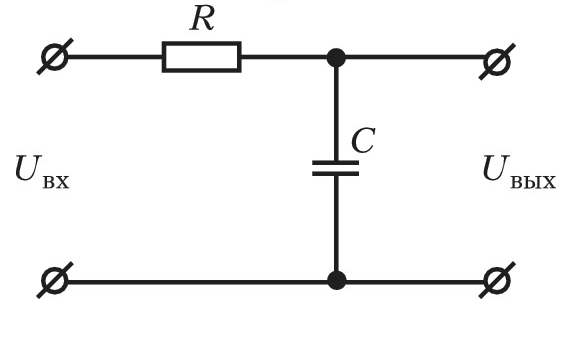
\includegraphics[width=0.4\textwidth]{int}
	\end{center}
	\vspace{-20pt}
	\caption{Интегрирующая ячейка --- RC-цепочка}
	\vspace{-10pt}
\end{wrapfigure}

Таким образом, для определения $B$ нужно проинтегрировать сигнал, наведенный переменным магниным полем на катушку. 

Для интегрирования сигнала применяют разного рода интегрирующие схемы. Простейшая из них состоит из соедниненных последовательно резистора $R$ и конденсатора $C$ и выполняет свое назначение, если сопротивление резистора $R$ сильно превышает сопротивление конденсатора (если выходной сигнал много меньше входного $U_{\textit{вых}} \ll U_{\textit{вх}}$). 

\begin{equation}
U_{\textit{вых}} = \frac{q}{C} =\frac{1}{C} \int Idt \simeq \frac{1}{RC} \int U_{\textit{вх}} dt.
\end{equation}

Этот вывод тем ближе к истине, чем больше постоянная времени $\tau = RC$ превосходит характерное время процесса. Для синусоидальных напряжений 
\begin{equation}
U_{\textit{вых}} = \frac{U_{\textit{вх}}}{RC\Omega},
\end{equation}
где $\Omega$ - частота сигнала. Отсюда итоговая формула
\begin{equation}
|B| = \frac {1}{SN} \int \mathscr{E}dt = \frac {1}{N} \int U_{\textit{вх}} dt = \frac{RC}{SN} \cdot U_{\textit{вых}} = \frac{RC}{SN} \cdot U_y.
\end{equation}
Для исследования зависимости $B(H)$ ферромагнитных материалов обычно используют образцы тороидальной формы. Подробное рассмотрение теории позволяет получить уравнение:
\begin{equation}
H = \frac{IN_0}{2\pi R} = \frac{U_x N_0}{R_0\cdot 2\pi R}
\end{equation}

\section*{Экспериментальная установка}
	\begin{center}
	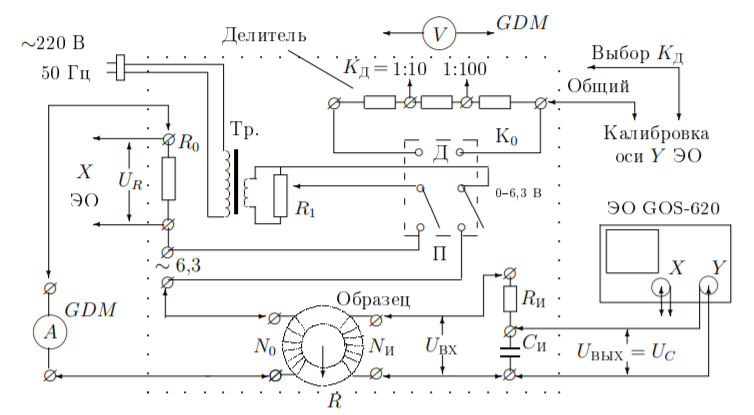
\includegraphics[width=\textwidth]{sch}
\end{center}

\section*{Экспериментальные данные и их обработка}
Для трех образцов: Fe-Si (кремнистое железо), Феррита и Fe-Ni (Пермаллой) были найдены растущие последовательности петель гистерезиса, в которых поля внутри образцов меняются от незначительных до приводящих вещества в состояния полного насыщения. Основные параметры системы и характеристики образцов:
\begin{itemize}
	\item 1. $R_0$ = 0.3 Ом; $\;R$ = 20 кОм; $\;C$ = 20 мкФ
	\item 2. (Fe-Ni): $\;N_0$ = 40; $\;N_U$ = 200; $\;S$ = 3.8 см; $\;2\pi R$ = 24 см
	\item 3. (Fe-Si): $\;N_0$ = 35; $\;N_U$ = 350; $\;S$ = 1.2 см; $\;2\pi R$ = 10 см
	\item 4. Феррит: $\;N_0$ = 35; $\;N_U$ = 400; $\;S$ = 3.0 см; $\;2\pi R$ = 25 см	
\end{itemize}
Графики соответствующих петель приведены на рисунках 3-5. Найденные исследуемые в эксперименте величины приведены в таблице 1.
\newpage
\begin{figure}[h!]
	\vspace{-1.7cm}
	\hspace{-1cm}
	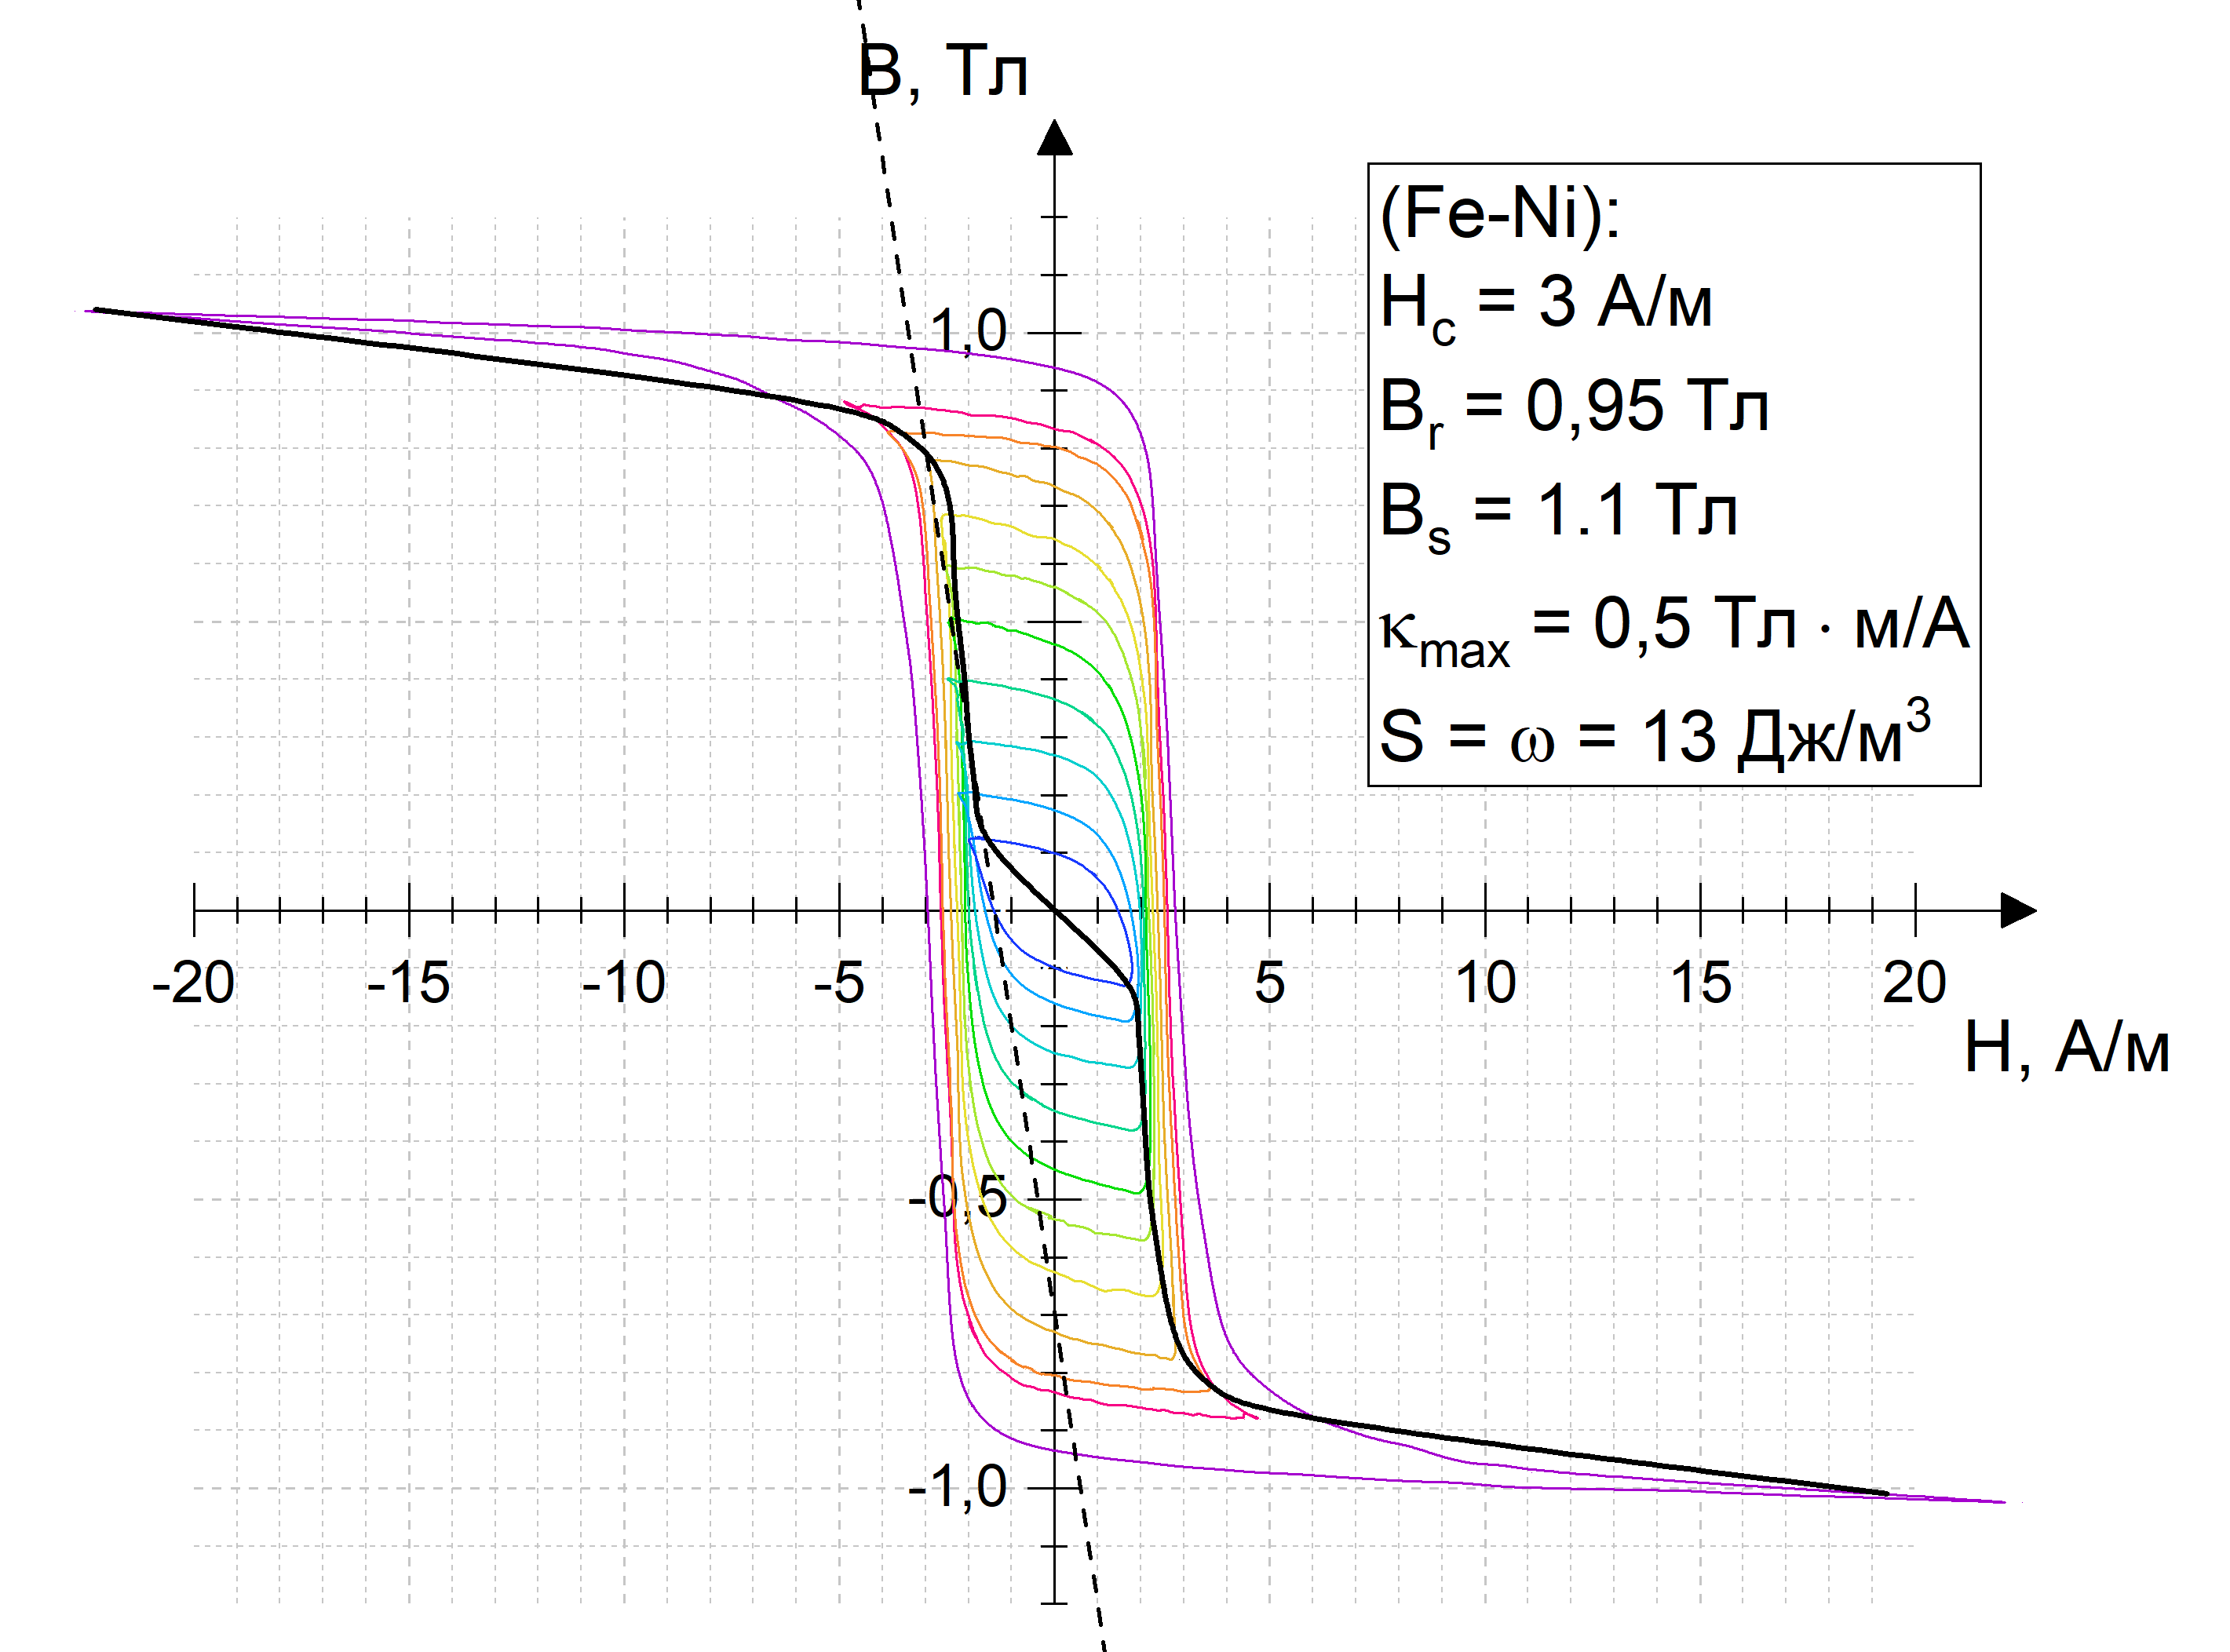
\includegraphics[width=1.05\textwidth]{FeNi.png}
	\vspace{-0.7cm}
	\caption{График зависимости $B(H)$ для $FeNi$}
		\vspace{-0.85cm}
\end{figure}
\begin{figure}[h!]

	\hspace{-1cm}
	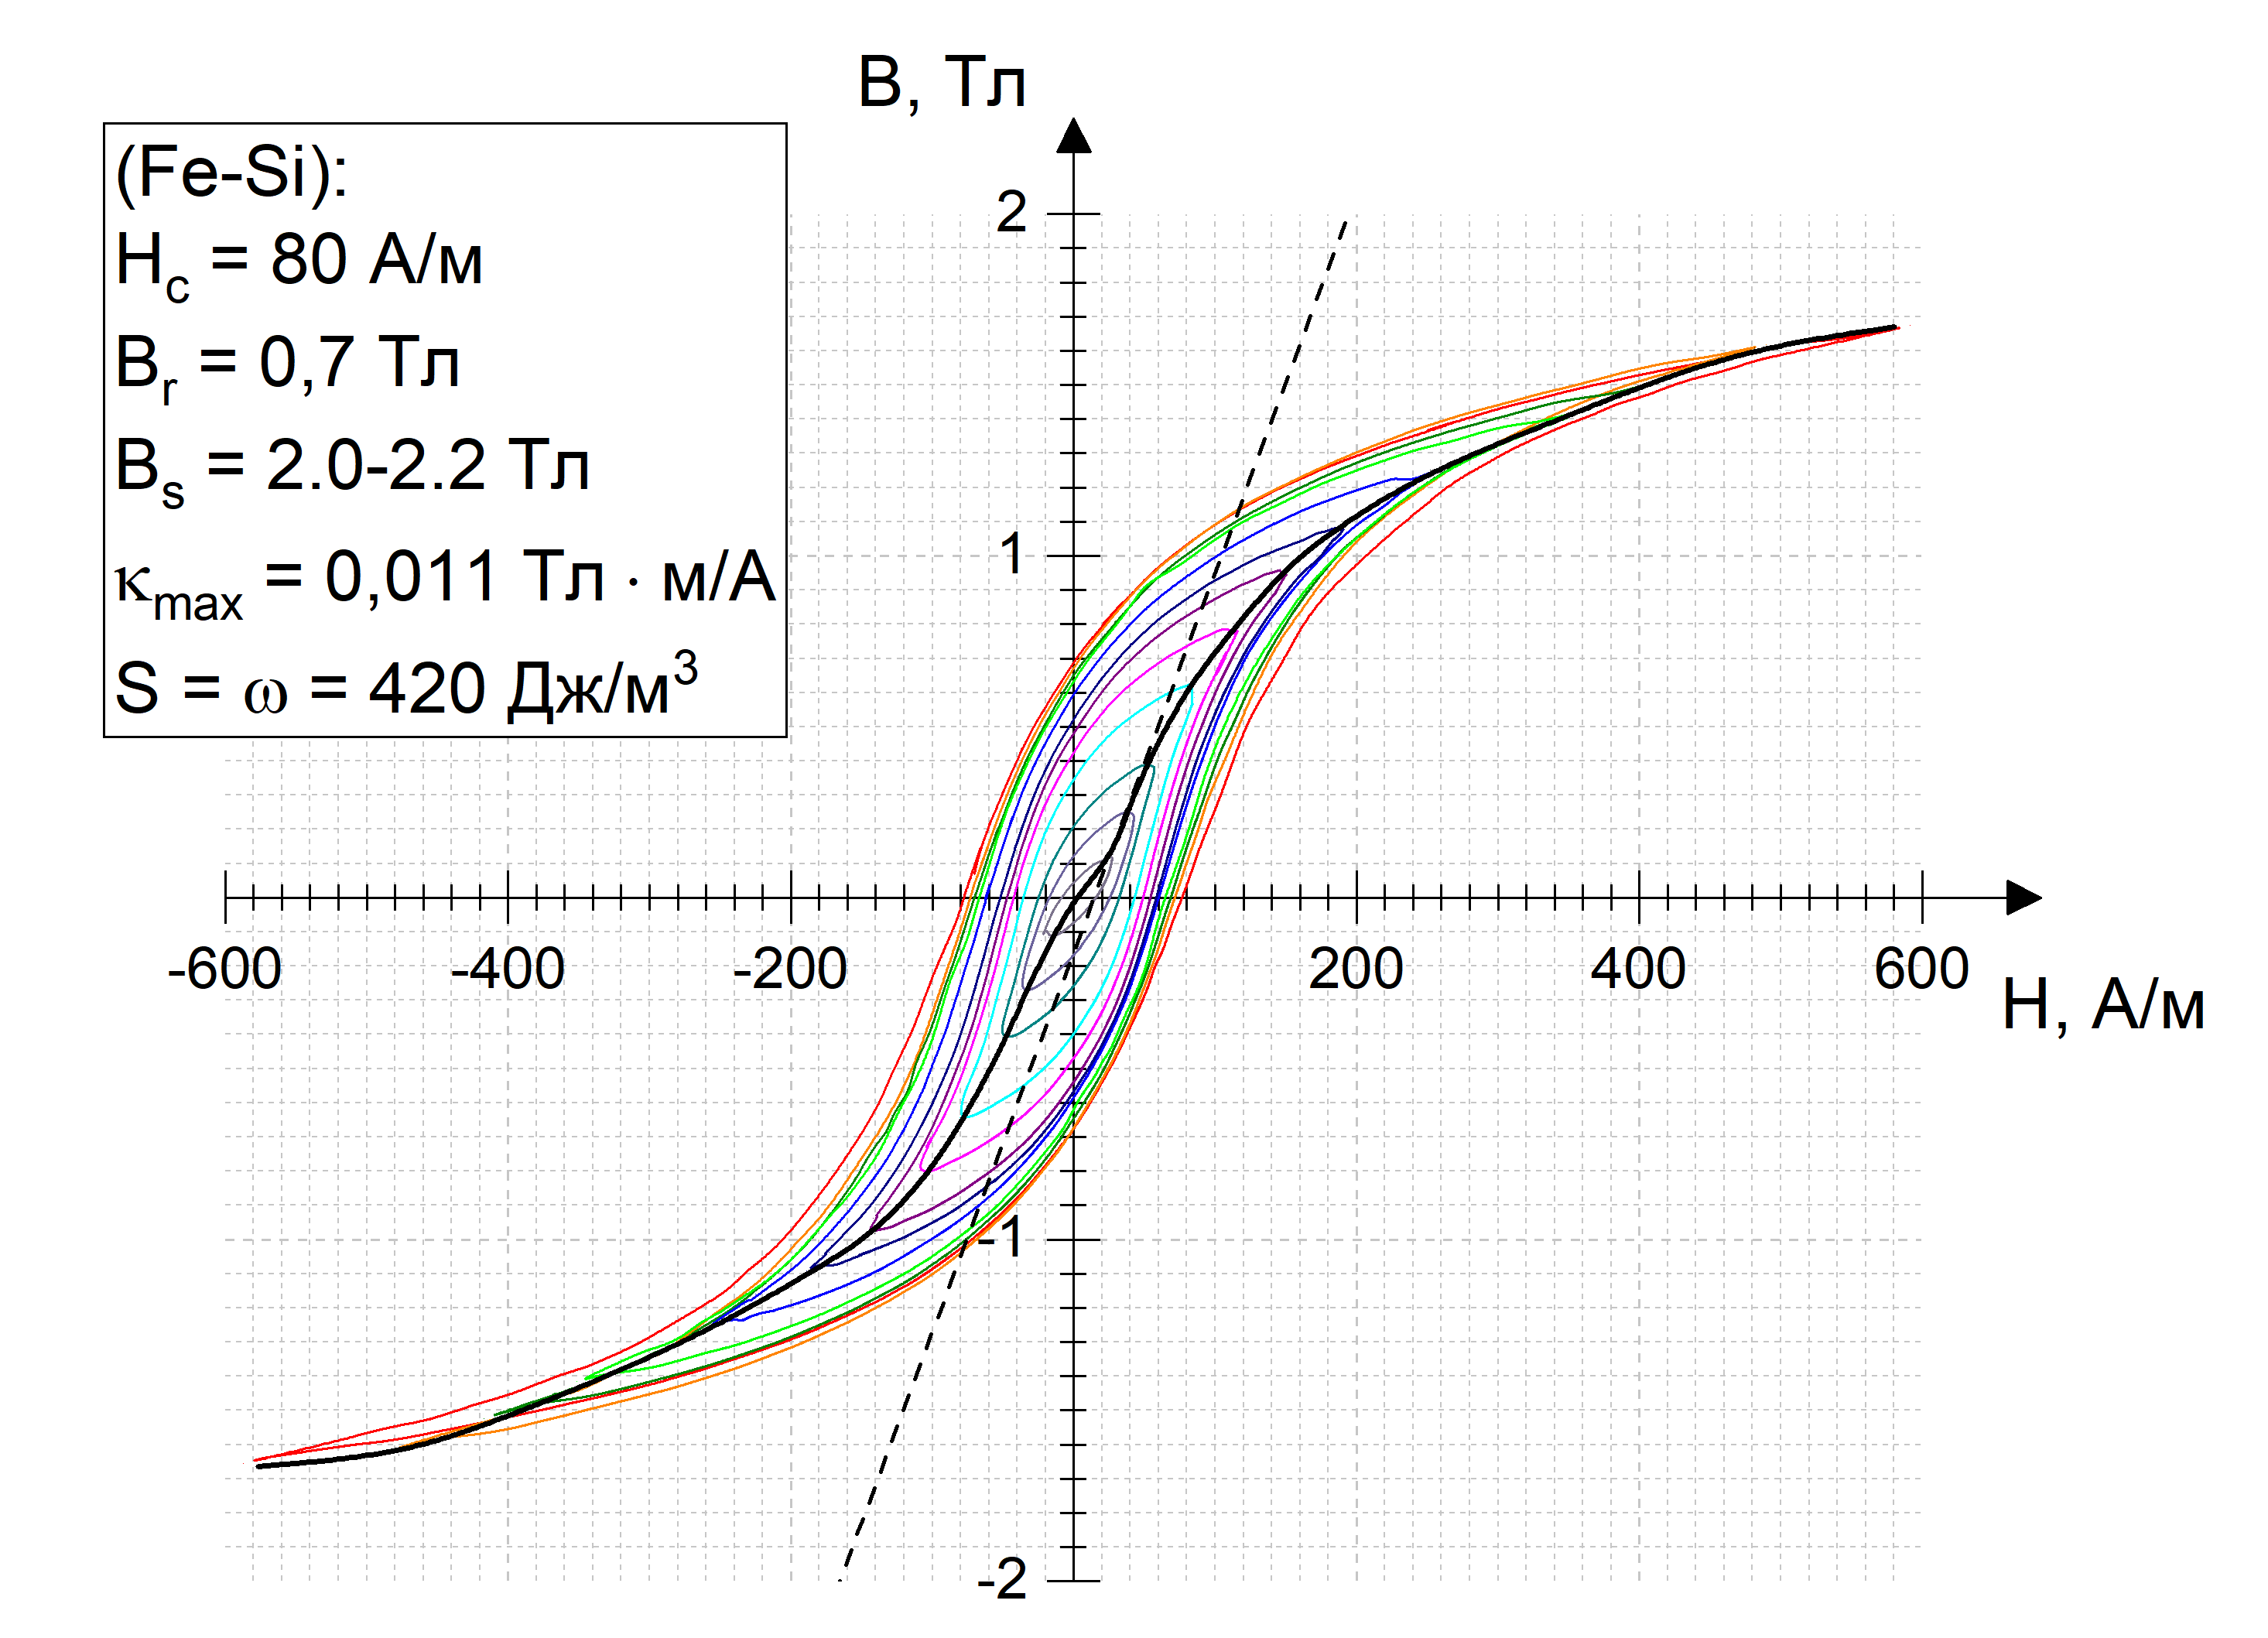
\includegraphics[width=1.05\textwidth]{FeSi.png}
		\vspace{-1.2cm}
	\caption{График зависимости $B(H)$ для $FeSi$}
\end{figure}
\newpage

\begin{figure}[h!]
	\vspace{-1.7cm}
	\hspace{-1cm}
	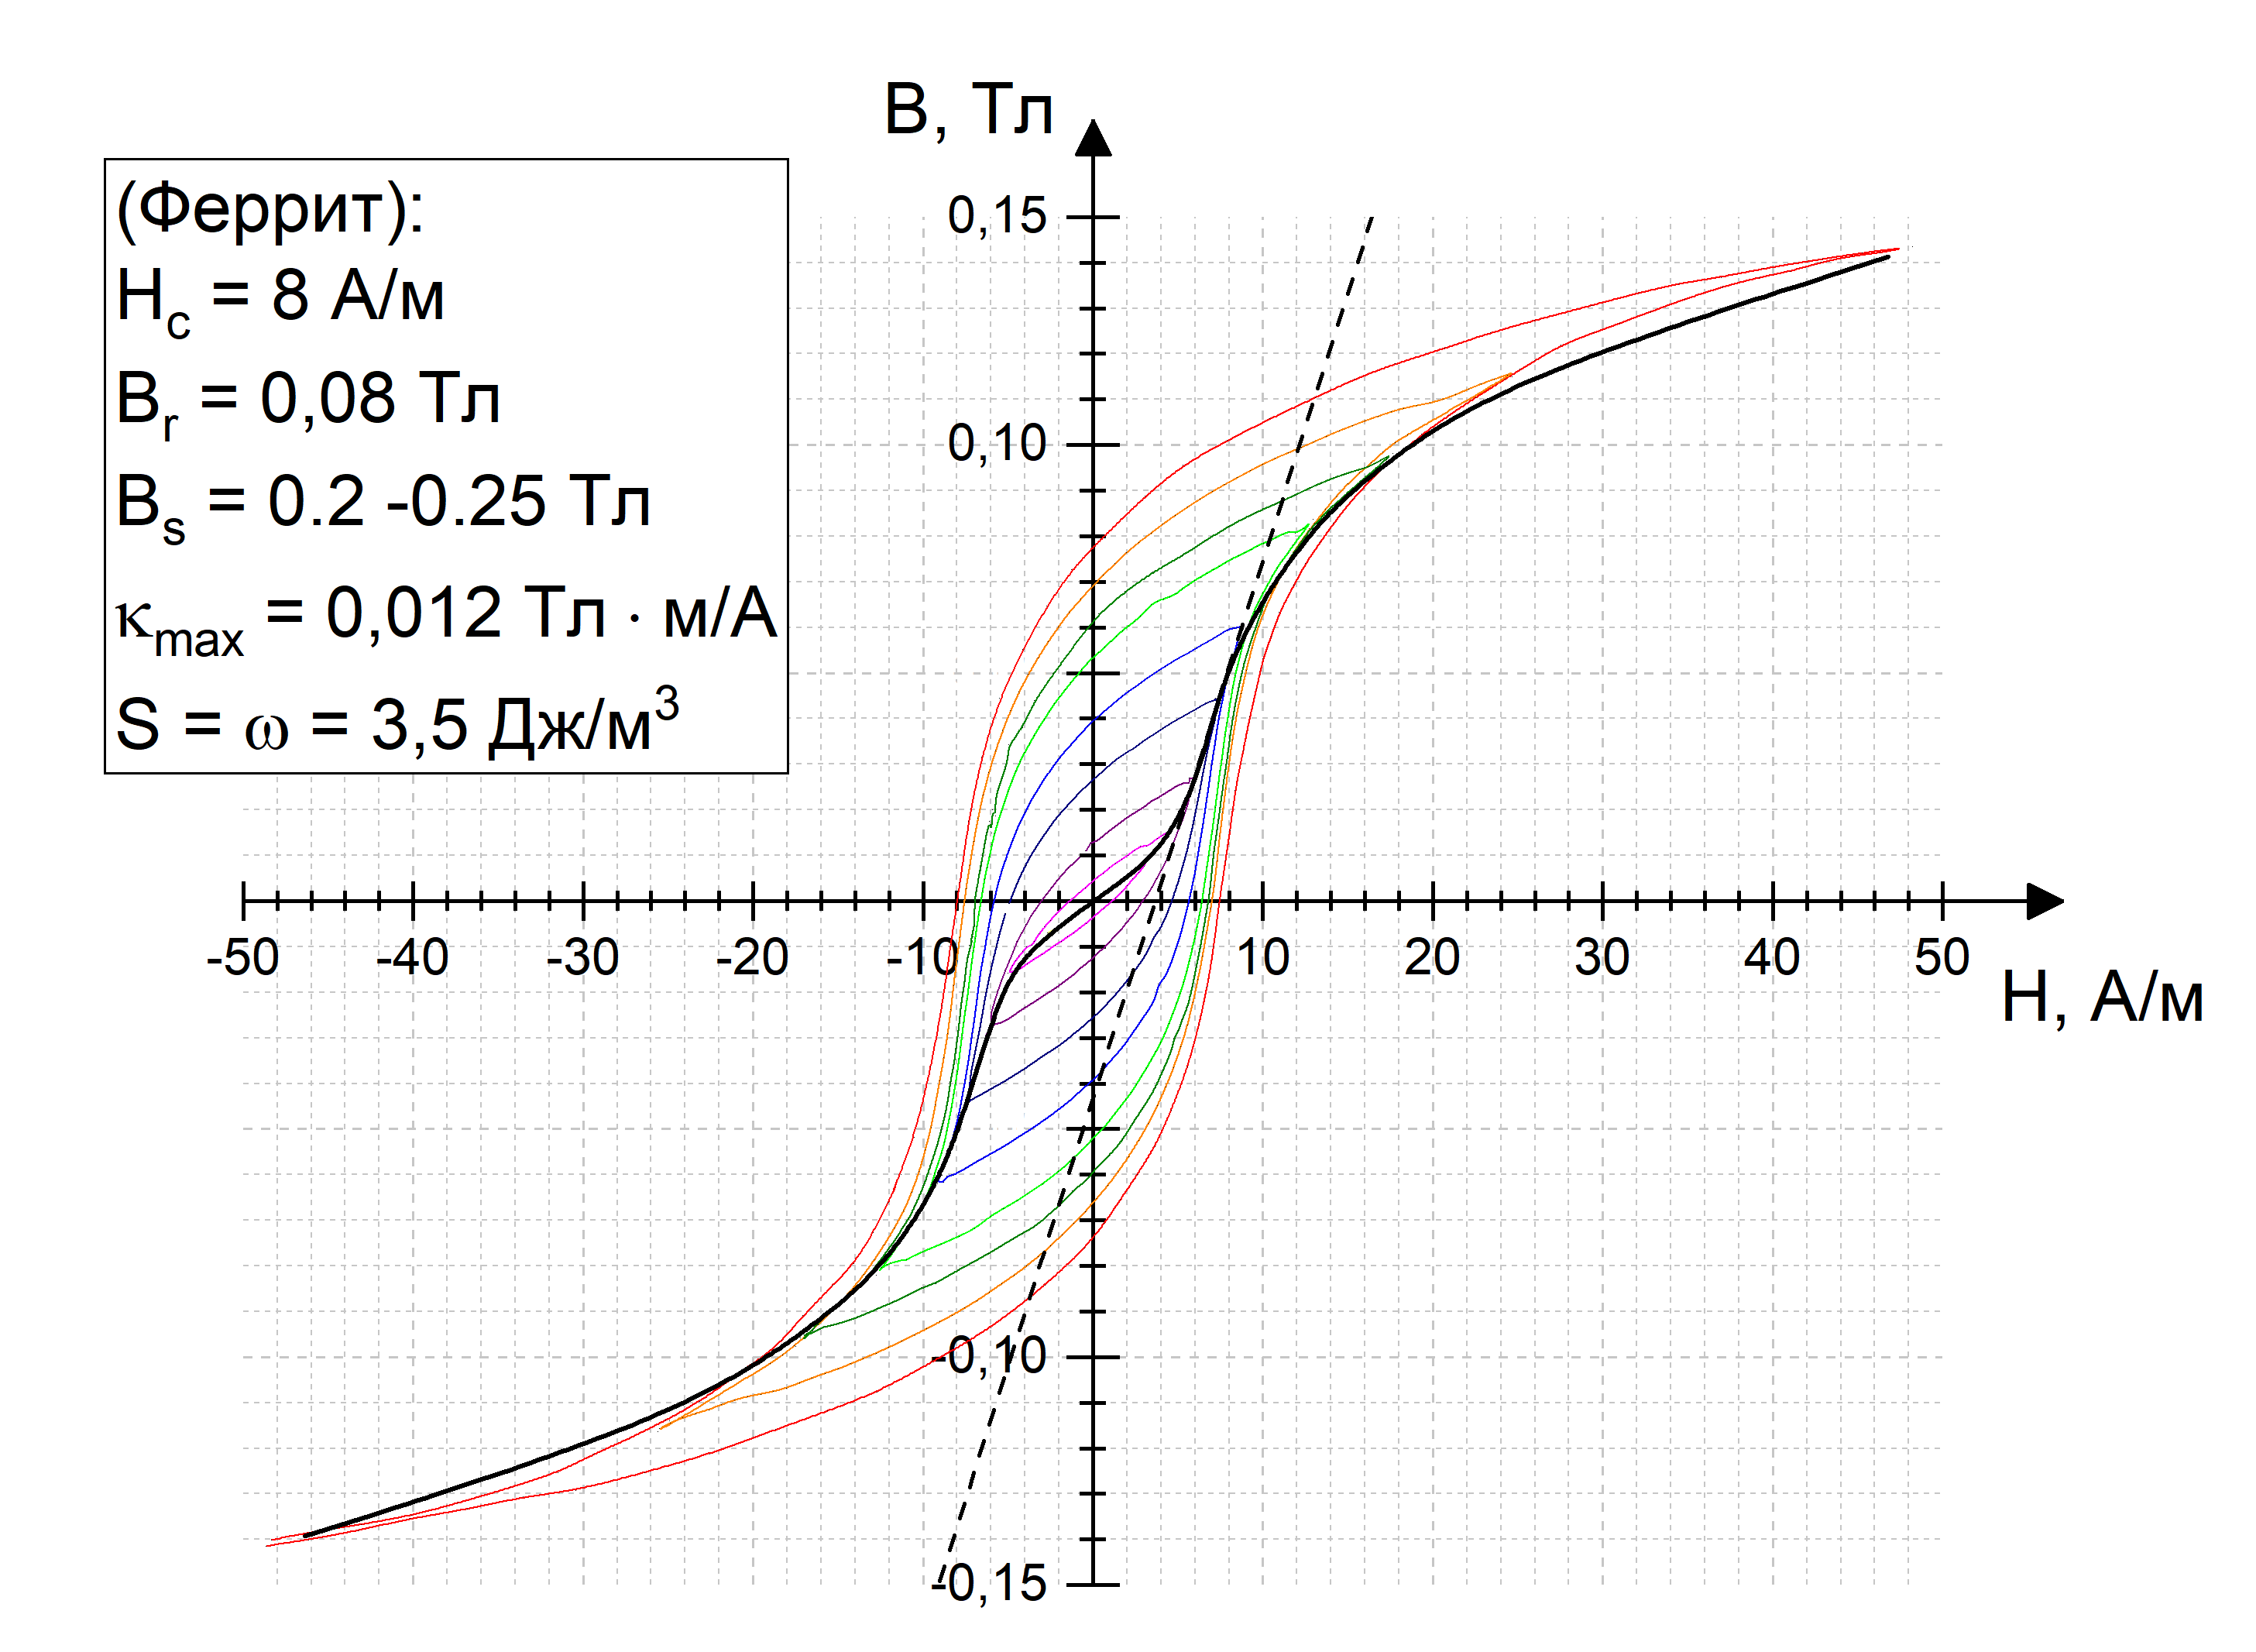
\includegraphics[width=1.05\textwidth]{Ferrit.png}

	\caption{График зависимости $B(H)$ для Феррита}
\end{figure}

\begin{table}[h!]
	\caption{Значения исслюдеуемых в работе величин}
	\vspace{0.5cm}
	\begin{tabular}{c|c|c|c|c|c|c|c|c|c|}
		\cline{2-10}
		& \multicolumn{6}{c|}{\begin{tabular}[c]{@{}c@{}}Экспериментальнае\\   значения\end{tabular}}                                                            & \multicolumn{3}{c|}{\begin{tabular}[c]{@{}c@{}}Табличные\\ значения\end{tabular}} \\ \cline{2-10} 
		& $H_c$, $\frac{\text{А}}{\text{м}}$ & $B_r$, Тл               & $B_s$, Тл                   & $\kappa_{max}$, Тл$\cdot \frac{\text{м}}{\text{А}}$       & $\mu_{max}$, ед. Си & $w$, $\frac{\text{Дж}}{\text{м}^3}$ & $H_c$, $\frac{\text{А}}{\text{м}}$              & $\mu_{max}$, ед. Си              &  $B_s$, Тл       \\ \hline
		\multicolumn{1}{|c|}{Fe-Ni}    & 3                      & 0.95                 & 1.1                      & 0.5                      & 4 $\cdot 10^6$                    & 13                         & 4                      & 1 $\cdot 10^6$                             & 1.08                 \\ \hline
		\multicolumn{1}{|c|}{Fe-Si}    & \multirow{2}{*}{80}    & \multirow{2}{*}{0.7} & \multirow{2}{*}{2.0-2.2} & \multirow{2}{*}{0.011} & \multirow{2}{*}{8.5 $\cdot 10^3$} & \multirow{2}{*}{420}       & 8                     & 40 $\cdot 10^3$                             & 2.0                  \\ \cline{1-1} \cline{8-10} 
		\multicolumn{1}{|c|}{Fe(техн)} &                        &                      &                          &                        &                       &                            & 80                    & 5 $\cdot 10^3$                              & 2.15                 \\ \hline
		\multicolumn{1}{|c|}{Феррит}   & 9                      & 0.08                 & 0.2-0.25                 & 0.012                  & 9.6 $\cdot 10^3$                & 3.5                        & 8-600                 & (3-10)$\cdot 10^3$                        & 0.2-0.4              \\ \hline
	\end{tabular}
\end{table}

\section*{Вывод.}
На основании имеющихся данных можно сделать несколько выводов. Во-первых, сравнивая значения  максимальной проницаемости и коэрцивной силы для кремнистого и технического железа, можно прийти к заключению, что в исследуемом образце в состав сплава входит ощутимое количество примеси, либо же содержание кремния в вещества больше чем предполгается в таблице(3$\%$). Во-вторых, довольно сильно отличаются значения максимальной проницаемости для пермаллоевого образца. Причина этого, увы, остается загадкой. В третьих, полученные значения для образца из феррита с хорошей степенью точности сходятся с табличными.	
\end{document}